\definecolor{carmine}{rgb}{0.4, 0.2, 0.09}
\begin{figure}[!ht]
    \centering
    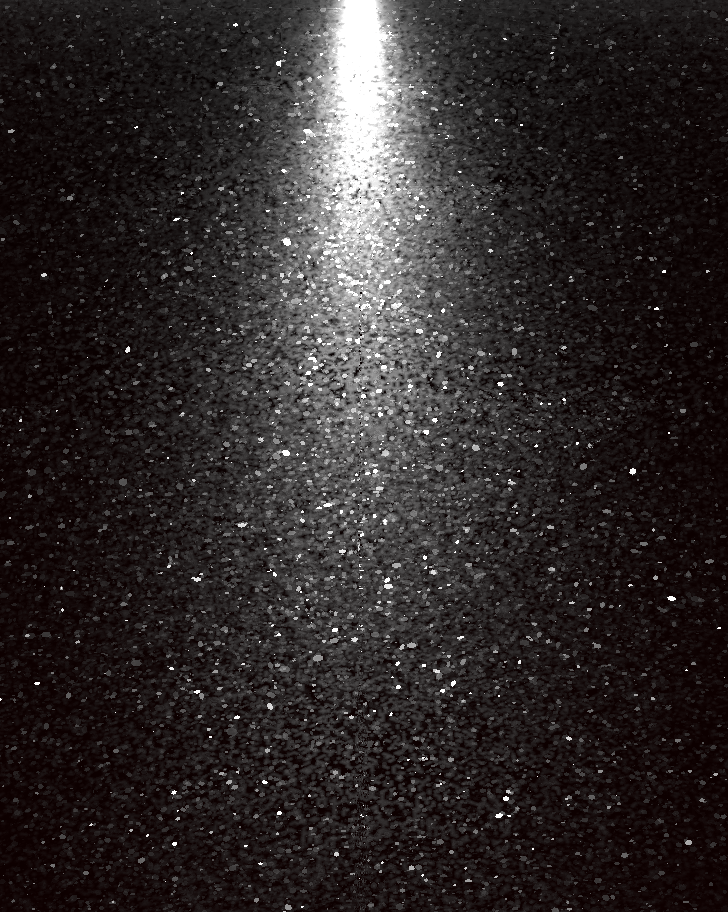
\includegraphics[width=0.4\linewidth]{anisotropy.png}%
    \begin{tikzpicture}
        \node[anchor=south west, inner sep=0] (image) at (0,0) {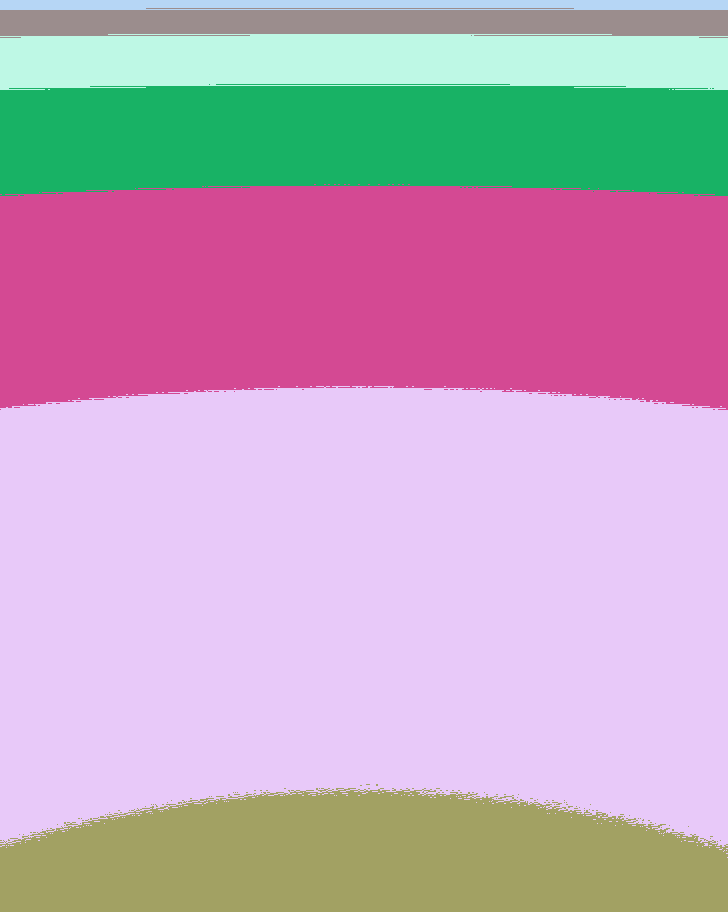
\includegraphics[width=0.4\linewidth]{anisotropy-levels.png}};
        \begin{scope}[x={(image.south east)},y={(image.north west)},color=carmine]
            \node at (0.5, 0.13) {$2\times$};
            \node at (0.5, 0.58) {$4\times$};
            \node at (0.5, 0.8) {$8\times$};
            \node at (0.5, 0.9) {$16\times$};
        \end{scope}
    \end{tikzpicture}
    \caption{Left: Glinty plane viewed at an angle of $1^{\circ}$ exposing high levels of anisotropy. Right: The respective anisotropy levels visualized using random colors.\label{fig:anisotropy}}
\end{figure}